\section{Gruppen}
%
%
%
\subsection{Definition:}
Eine Gruppe $G$ sei eine Menge mit einer Verknüpfung $* \ G \times G \rightarrow G$ derart, dass gilt:\\
\begin{description}
	\item[(1) Assoziativität:] $(a*b)*c = a*(b*c)$
	\item[(2) Neutrales Element:] $\exists e \in G | a*e=a=e*a \ \forall a \in G$ \\
						($e$ ist eindeutig: "`$e_{1}=e_{1}*e_{2}=e_{2}$"')
	\item[(3) Inverse:] Zu jedem $a \in G$ exsitiert ein $b \in G$ mit $a*b=e=b*a$\\
				(das $b$ wird als $a^{-1}$ bezeichnet, da es eindeutig von $a$ abhängt: \\
				"`$b_{1} = b_{1}*e=b_{1}(*a*b_{2})=(b_{1}*a)*b_{2}=e*b_{2}=b_{2}$"')
	\item[Beachte:] (1) und (2) sind Eigenschaften für einen Monoid
\end{description}
$G$ heiße zusätzlich kommutativ, falls gilt: $a*b=b*a \ \forall a,b \in G$
%
%
%
\subsection{Beispiel:}
\begin{description}
	\item[(a)] $\mathbb{N}$ mit + ist Monoid, aber keine Gruppe\\
			$\mathbb{Z}, \mathbb{Q},  \mathbb{R}$ bzgl. + sind Gruppen.\\
			$\mathbb{Z}/n\mathbb{Z}$ bzgl. + ist eine Gruppe (vererbt von $\mathbb{Z}$)\\
			$\mathbb{Z} \diagdown \{0\}$ bzgl. $\cdot$ ist Monoid\\
			$(\mathbb{Z}/n\mathbb{Z}) \diagdown \{0\}$ bzgl. $\cdot$ ist Gruppe $\Leftrightarrow n$ ist eine Primzahl\\
			Diese Regeln sind Kommutativ
	\item[(b)] Sei $\Omega$ eine Menge. Dann ist Abb $(\Omega, \Omega) = \{f|f:\Omega \rightarrow \Omega\}$ bzgl. 
			Komposition von Abbildungen immer im Monoid. Die Mege Sym$(\Omega) = \{f \in$ Abb. $(\Omega, \Omega)|
			f$ bijektiv$\}$ ist eine Gruppe bzgl. Komposition. "`symmetiche Gruppe"' Sym ($\Omega$) ist nicht 
			kommutativ, sofern $|\Omega| \geq 3$
	\begin{figure} [H]
		\centering
		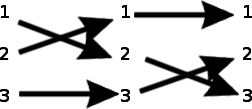
\includegraphics[width=4cm, height=2cm]{mainmatter/chapter3/pics/fadendia1-3.png}
		\caption{Fadendiagramm mit der Funktion 1 auf 3} 
	\end{figure}
	\begin{figure} [H]		
		\centering
		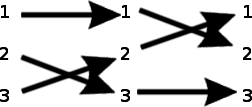
\includegraphics[width=4cm, height=2cm]{mainmatter/chapter3/pics/fadendia1-2.png}
		\caption{Fadendiagramm mit der Funktion 1 auf 2} 
	\end{figure}			
			In folgenden lassen wir $*$ weg.
\end{description}
%
%
%
\subsection{Lemma:}
Sei $G$ eine Gruppe und $a,b,c \in G$:
\begin{description}
	\item[(a)] $(ab)^{-1} = b^{-1}a^{-1}$ und $(a^{-1})^{-1} = a$, $e^{-1}=e$
	\item[(b)] Setzt man $a^{0}=e$, $a^{n}=a(a^{n-1})$ und $a^{-n} = (a^{-1})^{n}$ \ $\forall n \geq 1$ so gelten die 
			üblichen Potenzgesetze.
\end{description}
Kurzregeln:
\begin{description}
	\item[-] aus $ab=ac$ folgt stets $b=c$ (Multiplikation mit $a^{-1}$ von links)
	\item[-] aus $ab=cb$ folgt stets $a=c$ (Multiplikation mit $b^{-1}$ von rechts)
\end{description}
%
%
%
\subsection{Definition:}
Eine Untergruppe $U$ der Gruppe $G$ sei eine Teilmenge von $G$, die bzgl. der Verknüpfung (Multiplikation) in $U$ selbst eine Gruppe bildet. d.h. es musst gelten:
\begin{description}
	\item[-] $e \in U$
	\item[-] $U$ ist gegen Multiplikation abgeschlossen und gegen Inversion. (Dies ist gewähtleistet, falls für alle $a,b \in U$ 
			gilt $ab^{-1} \in U$
\end{description}
Schreibe: $U \leq G$
%
%
%
\subsection{Beispiel:}
\begin{description}
	\item[(a)] $\mathbb{Z} \leq \mathbb{Q}$ bzgl. +
	\item[(b)] $\{a^{2}|a \in (\mathbb{Z}/n\mathbb{Z})^{x}\} \leq (\mathbb{Z}/n\mathbb{Z})^{x}$ (bzgl. $\cdot$)
			da $1^{2} = 1$, $a^{2}b^{2} = aabb$, $abab = (ab)^{2}$,\\
			 $(a^{2})^{-1} = (a^{-1})^{2}$
\end{description}
%
%
%
\subsection{Satz von Lagrange}
Sei $G$ endliche Gruppe und $U \leq G$. Dann $|U|$ \Large{|} \normalsize{$|G|$}.
\begin{description}
	\item[Beweis:] \quad\\
	\item[] Die Rechtsmultiplikation mit festen $g \in G$ ist eine bijektive Abbildung $G \rightarrow G$ /* $x \rightarrow x 
		\cdot g$ (die Inverse ist Rechtsmultiplikativ mit $g^{-1}$)
	\item[] Daher gilt $|U| = |U \cdot g|$, $U \cdot g = \{u \cdot g|u \in U\}$ für jedes (feste) $g \in G$
\end{description}
\quad\\
$\mathbb{Z} = \mathop{\dot{\bigcup}}\limits^{n-1}_{k = 0} \ (k+n \ \mathbb{Z})$\\
\quad\\
$G = \mathop{\bigcup}\limits_{g \in G} \ U \cdot g$,  da $g = e \cdot g \in U \cdot g$\\
\quad\\
Zeige: Die $Ug$ ($g$ geeignet) bilden eine Partition von G. (dann:\\
 $|G| = | \mathop{\bigcup}\limits_{g \textrm{ geeignet}} \ Ug| = \sum\limits_{g\textrm{ geeignet}}|Ug| = \sum\limits_{g\textrm{ geeignet}} |U| = m \cdot |U|$ wo $m =$ Anzahl der $Ug$ ($g$ geeignet))\\
\quad\\
Dazu sei $x \in Ug_{1} \cap Ug_{2}$ Zeige: $Ug_{1} = Ug_{2}$\\
Dann $u_{1}g_{1} \cdot x = u_{2}g_{2}$ mit $u_{1}, u_{2} \in U$ geeignet
\begin{equation*}
	\Rightarrow U \cdot u_{1}g_{1} = U \cdot u_{2}g_{2}
\end{equation*}
\begin{equation*}
	\Leftrightarrow Ug_{1} = Ug_{2}
\end{equation*}
%
%
%
\subsection{Folgerung:}
In jeder endlichen Gruppe $G$ gilt: $g^{|G|} = e \ \forall g \in G$ (vgl. Satz von Euler (II.2.6), wo $(\mathbb{Z}/n\mathbb{Z})^{x} = \varphi(n)$ war)
\begin{description}
	\item[Beweis:] \quad\\
			Betrachte $U=\{g^{z}|z \in \mathbb{Z}\} \leq G$ für festes $g$ aus $G$. \\
			Zeige: $g^{|U|} = e$ (dann $g^{|G|}=(g^{|U|})^{m}=e$ für $|G| = |U| \cdot m$ gemäß 1.6)\\
			Kopiere hierzu den Beweis des Satzes von Euler und verwende, dass $U$ kommutativ ist.
\end{description}
%
%
%
\subsection{Definition:}
Ein Gruppenhomomorphismus $\varphi: G \rightarrow H$ (wobei $G,H$ Gruppen sind) Sei eine Abbildung mit $\varphi(a \cdot b) = \varphi (a) \cdot \varphi (b) \ \forall a,b \in G$
%
%
%
\subsection{Satz:}
\begin{description}
	\item[(a)] $\varphi(e)=e$ \qquad $\varphi(a^{-1}) = (\varphi(a))^{-1}$ \qquad\ $\forall \ a \in G \ \checkmark$
	\item[(b)] Bild $q \leq H \ \checkmark$
	\item[(c)] Die Fasern von $\varphi$ sind genau die Menge $Ug \ (g \in G)$\\
			wo $N=\{u \in G|\varphi(u)=e\}=:$ Kern $\varphi$\\
			und $Ng = \{ug|u \in N\}$
	\item[(d)] $N$ ist ein Normalteiler von $G$, d.h.\\
	\begin{description}
		\item[-] $N \leq G$ und
		\item[-] $g^{-1}ug \in N$ für jedes $u \in N$ und $g \in G$
	\end{description}
	\item[Beweis:] \quad
	\begin{description}
		\item[(c):] Sei $g \in G$ fest. Betrachte $\varphi(g) \in$ Bild $\varphi$\\
				Sei $a \in G$ mit $\varphi(a) = \varphi(g)$\\
				Dann:	
				\begin{description}
					\item[]$e = \varphi(a)\varphi(g)^{-1}=\varphi(a \cdot g^{-1})$ und $a \cdot g^{-1} \in$ 
						Kern $\varphi=N$
					\item[]$a \cdot g^{-1}= u \in N$ für ein $u$
					\item[]$\Rightarrow a=u \cdot g \in Ng$
				\end{description}
				Dies zeigt: Faser zu $\varphi(g)$ ist in $Ng$ enthalten.\\
				Sei umgekehrt $a \in Ng$, also $a= u \cdot g$ für ein $u \in N =$ Kern$\varphi$\\
				$\Rightarrow \varphi(a)=\varphi(u \cdot g) = \varphi(u) \cdot \varphi(g) = e \cdot \varphi(g) = 
				\varphi(g)$\\
				$\Rightarrow a$ in Faser zu $\varphi(g)$
		\item[(d):] \quad
				\begin{description}
				\item[-] Nach (a) ist $e \in N$. Ferner gilt für $a,b \in N$:\\
						$\varphi(ab^{-1}) = \varphi(a) \cdot \varphi(b)^{-1} = e \cdot e^{-1} =e$\\
						$\Rightarrow ab^{-1} \in N$ Kern$\varphi$
				\item[-] Für $u \in$ Kern$\varphi$ und $g \in G$ gilt\\
					$\varphi(g^{-1}ug) = \varphi(g)^{-1} \cdot \mathop{\underbrace{\varphi(g)}}\limits_{=e} 
					\cdot \varphi(g) = \varphi(g)^{-1} \cdot \varphi(g) =e$\\
					$\Rightarrow g^{-1}ug \in N$
				\end{description}
	\end{description}
\end{description}
%
%
%
\subsection{Bemerkung}
Sei $\varphi: G \rightarrow H$ ein Gruppenhomomorphismus. Nach II.1.9(c) ist eine Projektion gegeben durch:
\begin{description}
	\item[] $Ng \longleftrightarrow \varphi(g)$
	\item[] $\{Ng|g \in G\} \mathop{\longleftrightarrow}\limits^{\tilde{\varphi}}$ Bild$\varphi$
\end{description}
Vermöge $\tilde{\varphi}$ übertragen wir die Gruppenstruktur von Bild$\varphi$ auf $\{Ng|g \in G\}  =: G/N$\\
Wie funktioniert die Multiplikation in $G/N$?
\begin{equation*}
	(Ng_{1})\cdot(Ng_{2}) \mathop{\longleftrightarrow}\limits^{\tilde{\varphi}} \varphi(g_{1}) \cdot 		
	\varphi(g_{2})=\varphi(g_{1}g_{2}) \mathop{\longleftrightarrow}\limits^{\tilde{\varphi}} N(g_{1}g_{2})
\end{equation*}
\begin{description}
	\item[Also:] $(Ng_{1})\cdot(Ng_{2}) =  N(g_{1}g_{2}) \quad \forall \ g_{1},g_{2} \in G$
	\item[Ebenso:] $Ne$ ist das neutrale Element in $G/N$\\
			$N(g^{-1})$ ist das Inverse zu $Ng$.
\end{description}
Das entspricht genau der Addition auf $\mathbb{Z}/n\mathbb{Z} = \{n\mathbb{Z}+k|k\in\mathbb{Z}\}$